%%%%%%%%%%%%%%%%%%%%%%%%%%%%%%%%%%%%%%%%%%%%%%%%%%%%%%%%%%%%%%%%%%%%%%%%%%%%%%%
% PLANTILLA DE PRESENTACIÓN BEAMER - WASAFF CONSULTING
% VERSIÓN 3.0: EDICIÓN FINAL DE ALINEACIÓN Y DISEÑO
% Resultado profesional, sin errores y con una composición equilibrada.
%%%%%%%%%%%%%%%%%%%%%%%%%%%%%%%%%%%%%%%%%%%%%%%%%%%%%%%%%%%%%%%%%%%%%%%%%%%%%%%

\documentclass[10pt, aspectratio=169]{beamer} % Ratio 16:9 ideal para pantallas y LinkedIn

% --- 1. TEMA Y CONFIGURACIÓN VISUAL ---
\usetheme{metropolis}

% --- Paquetes Esenciales ---
\usepackage[utf8]{inputenc}
\usepackage[spanish]{babel}
\usepackage{graphicx}
\usepackage{qrcode}
\usepackage{tikz}

% --- 2. DEFINICIÓN DEL BRANDING WASAFF CONSULTING (TEMA CLARO) ---
\definecolor{WasaffNavy}{HTML}{001F3F}
\definecolor{WasaffCopper}{HTML}{B87333}

% --- Adaptación del tema a fondo blanco y colores de bloques ---
\setbeamercolor{background canvas}{bg=white}
\setbeamercolor{normal text}{fg=black!85} 
\setbeamercolor{frametitle}{bg=white, fg=WasaffNavy}
\setbeamercolor{alerted text}{fg=WasaffCopper}
\setbeamercolor{progress bar in head/foot}{bg=WasaffCopper, fg=white}
\setbeamercolor{title}{fg=WasaffNavy}
\setbeamercolor{subtitle}{fg=black!70}

\setbeamercolor{block title}{bg=WasaffNavy!10, fg=WasaffNavy}
\setbeamercolor{block body}{bg=WasaffNavy!5}
\setbeamercolor{block title alerted}{bg=WasaffCopper!10, fg=WasaffCopper}
\setbeamercolor{block body alerted}{bg=WasaffCopper!5}

% --- 3. COMANDO PERSONALIZADO PARA PLACEHOLDERS ---
\newcommand{\placeholderfigure}[2][5cm]{% 
  \begin{tikzpicture}
    \node[
      fill=gray!15, 
      minimum width=0.9\textwidth, 
      minimum height=#1, 
      text=gray!50, 
      font=\Huge\sffamily\bfseries
    ] at (0,0) {#2};
  \end{tikzpicture}
}

% --- 4. INFORMACIÓN DEL DOCUMENTO Y PORTADA ---
\title{Análisis de Caso: El Costo Oculto de la Simetría}
\author{Felipe Wasaff}
\institute{WASAFF CONSULTING}
\date{19 de agosto de 2025}
\logo{
\includegraphics[height=0.7cm]{wasaff_logo.png}}
% No usaremos titlegraphic para tener más control con la opción [standout]
% \titlegraphic{\placeholderfigure{A}} 

\begin{document}

% --- PORTADA ---
\begin{frame}[standout]
    \maketitle
    \vspace{0.5em}
    \large\alert{¿Tomaría una Decisión de Inversión Basada en un Error del 37\%?}
\end{frame}

% --- DIAPOSITIVA 2: EL ESCENARIO ---
\begin{frame}
  \frametitle{El Desafío: Un Manifold Crítico}
  
  \begin{columns}[T, totalwidth=\textwidth] 
    \begin{column}{0.45\textwidth}
      \begin{figure}
      \centering
        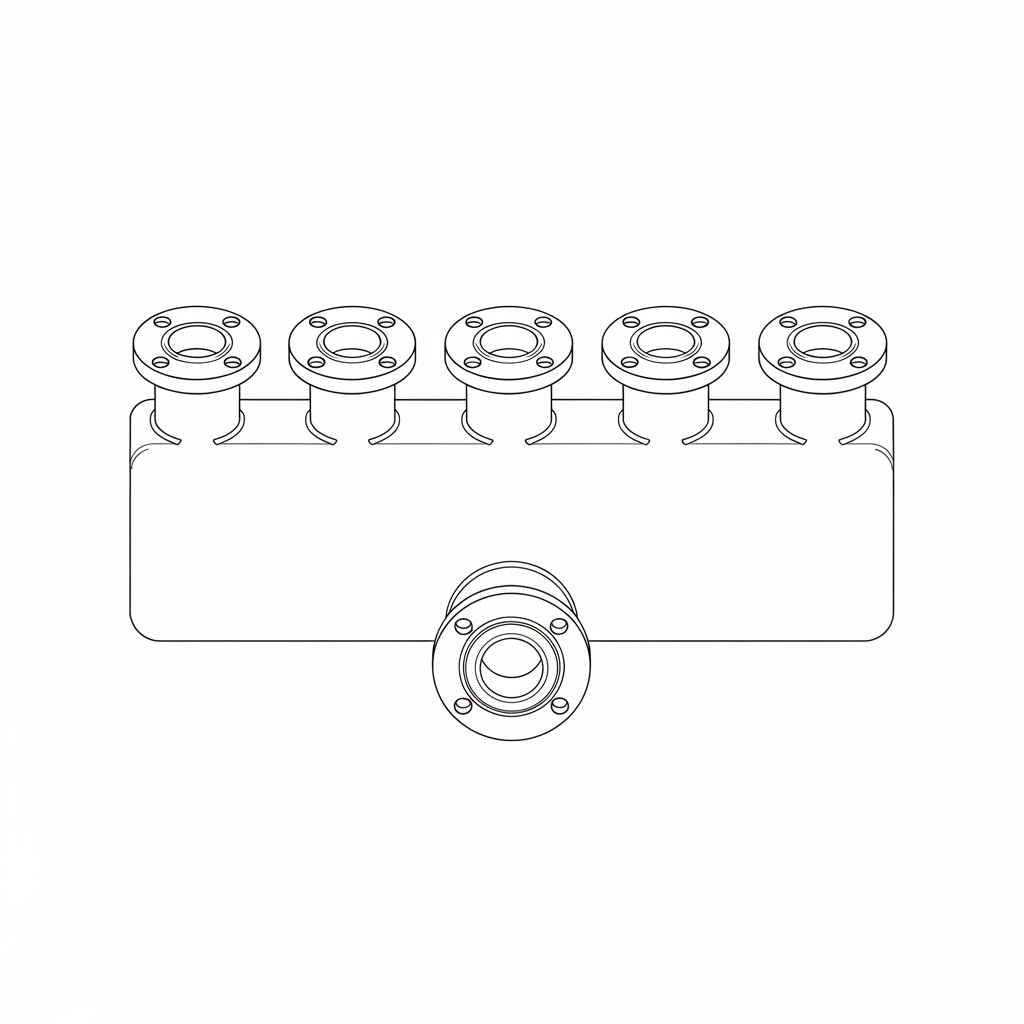
\includegraphics[scale=.2]{manifold_idealizado.png}
        \caption{Diseño del manifold basado en la suposición de simetría.}
      \end{figure}
    \end{column}
    \begin{column}{0.55\textwidth}
      \textbf{El Objetivo:} Asegurar que 5 equipos críticos reciban, cada uno, un 20\% del flujo de enfriamiento.
      \vspace{1.5em}
      
      \textbf{La Suposición:} Una geometría perfectamente simétrica producirá una distribución de flujo simétrica.
      \vspace{1.5em}
      
      \alert{Pusimos esta premisa a prueba con dos métodos.}
    \end{column}
  \end{columns}
\end{frame}

% --- DIAPOSITIVA 3: EL RESULTADO ESPERADO ---
\begin{frame}
  \frametitle{Método 1: La Respuesta de la "Experiencia"}
  \framesubtitle{El cálculo analítico-empírico}
  
  \begin{block}{Resultado del Análisis Empírico}
      El cálculo basado en correlaciones empíricas predice una distribución casi perfecta y una caída de presión de 0.0031 bar. Un diseño que, sobre el papel, \textbf{sería aprobado sin dudar.}
  \end{block}
  
  \vfill % Empuja el siguiente bloque hacia abajo
  
  \begin{block}{Veredicto del Método 1}
      \centering
      \Large \textbf{\textcolor{green!50!black}{Predicción: ¡El Diseño Funciona!}}
  \end{block}
\end{frame}

% --- DIAPOSITIVA 4: LA REALIDAD FÍSICA ---
\begin{frame}
  \frametitle{Método 2: La Realidad que Revela la Física}
  \framesubtitle{La simulación por primeros principios (CFD)}
  
  \begin{columns}[T, totalwidth=\textwidth]
    \begin{column}{0.55\textwidth}
      \begin{figure}
        \placeholderfigure[4cm]{C}
        \caption{La simulación muestra cómo el momento del fluido rompe la simetría.}
      \end{figure}
    \end{column}
    \begin{column}{0.45\textwidth}
      \textbf{Resultados Reales:}
      \begin{itemize}
        \item $\Delta P$ real: \textbf{0.0042 bar} \alert{(+37\%)}
        \item Flujo Salida 1: 28\%
        \item Flujo Salida 5: 14\%
      \end{itemize}
    \end{column}
  \end{columns}
  
  \begin{alertblock}{Veredicto del Método 2}
    \centering
    \large \textbf{Realidad: ¡El Diseño es Inherentemente Defectuoso!}
  \end{alertblock}
\end{frame}

% --- DIAPOSITIVA 5: IMPACTO EN EL NEGOCIO ---
\begin{frame}
  \frametitle{¿Qué Significa Realmente un Error del 37\%?}
  
  \begin{block}{Consecuencias de Negocio de un Diseño Basado en Suposiciones}
    \begin{itemize}
      \item<1-> \textbf{Activos Críticos en Riesgo:} La última salida recibe la mitad del flujo necesario. El equipo 5 se sobrecalentará, \alert{reduciendo drásticamente su vida útil}.
      \item<2-> \textbf{OPEX Disparado:} La bomba, dimensionada con una caída de presión subestimada, trabajará forzada, \alert{consumiendo hasta un 20\% más de energía}.
      \item<3-> \textbf{ROI Fallido:} La línea de producción NUNCA alcanzará su capacidad de diseño, \alert{invalidando el retorno de la inversión del proyecto}.
    \end{itemize}
  \end{block}
\end{frame}

% --- DIAPOSITIVA 6: TU FILOSOFÍA ---
\begin{frame}
  \frametitle{La Filosofía: De la Aproximación a la Certeza}
  \vfill
  \begin{center}
      
\includegraphics[height=1cm]{wasaff_logo.png}
  \end{center}
  \vspace{1em}
  
  \begin{block}{}
      \centering
      La "experiencia" se basa en promedios. Los primeros principios analizan \textbf{SU} realidad física.
      \vspace{1.5em}
      
      \large \alert{Antes de invertir en acero y equipos, invierta en certeza.}
      \vspace{1em}
      
      Es la única forma de garantizar el rendimiento de una inversión.
  \end{block}
  \vfill
\end{frame}

% --- DIAPOSITIVA 7: LA LLAMADA A LA ACCIÓN ---
\begin{frame}
  \frametitle{¿Tiene un Desafío Técnico Similar?}
  
  \begin{columns}[T, totalwidth=\textwidth]
    \begin{column}{0.6\textwidth}
      \textbf{Obtenga Claridad antes de Invertir.}
      \vspace{1em}
      
      Mi servicio de \textbf{Diagnóstico Estratégico de 10 Días} está diseñado para darle esta misma certeza física y financiera.
      \vspace{1em}
      
      El entregable es una \textbf{hoja de ruta cuantificada}.
      \vspace{2em}
      
      \Large\bfseries \href{https://www.wasaffconsulting.com}{www.wasaffconsulting.com}
    \end{column}
    \begin{column}{0.4\textwidth}
      \begin{figure}
		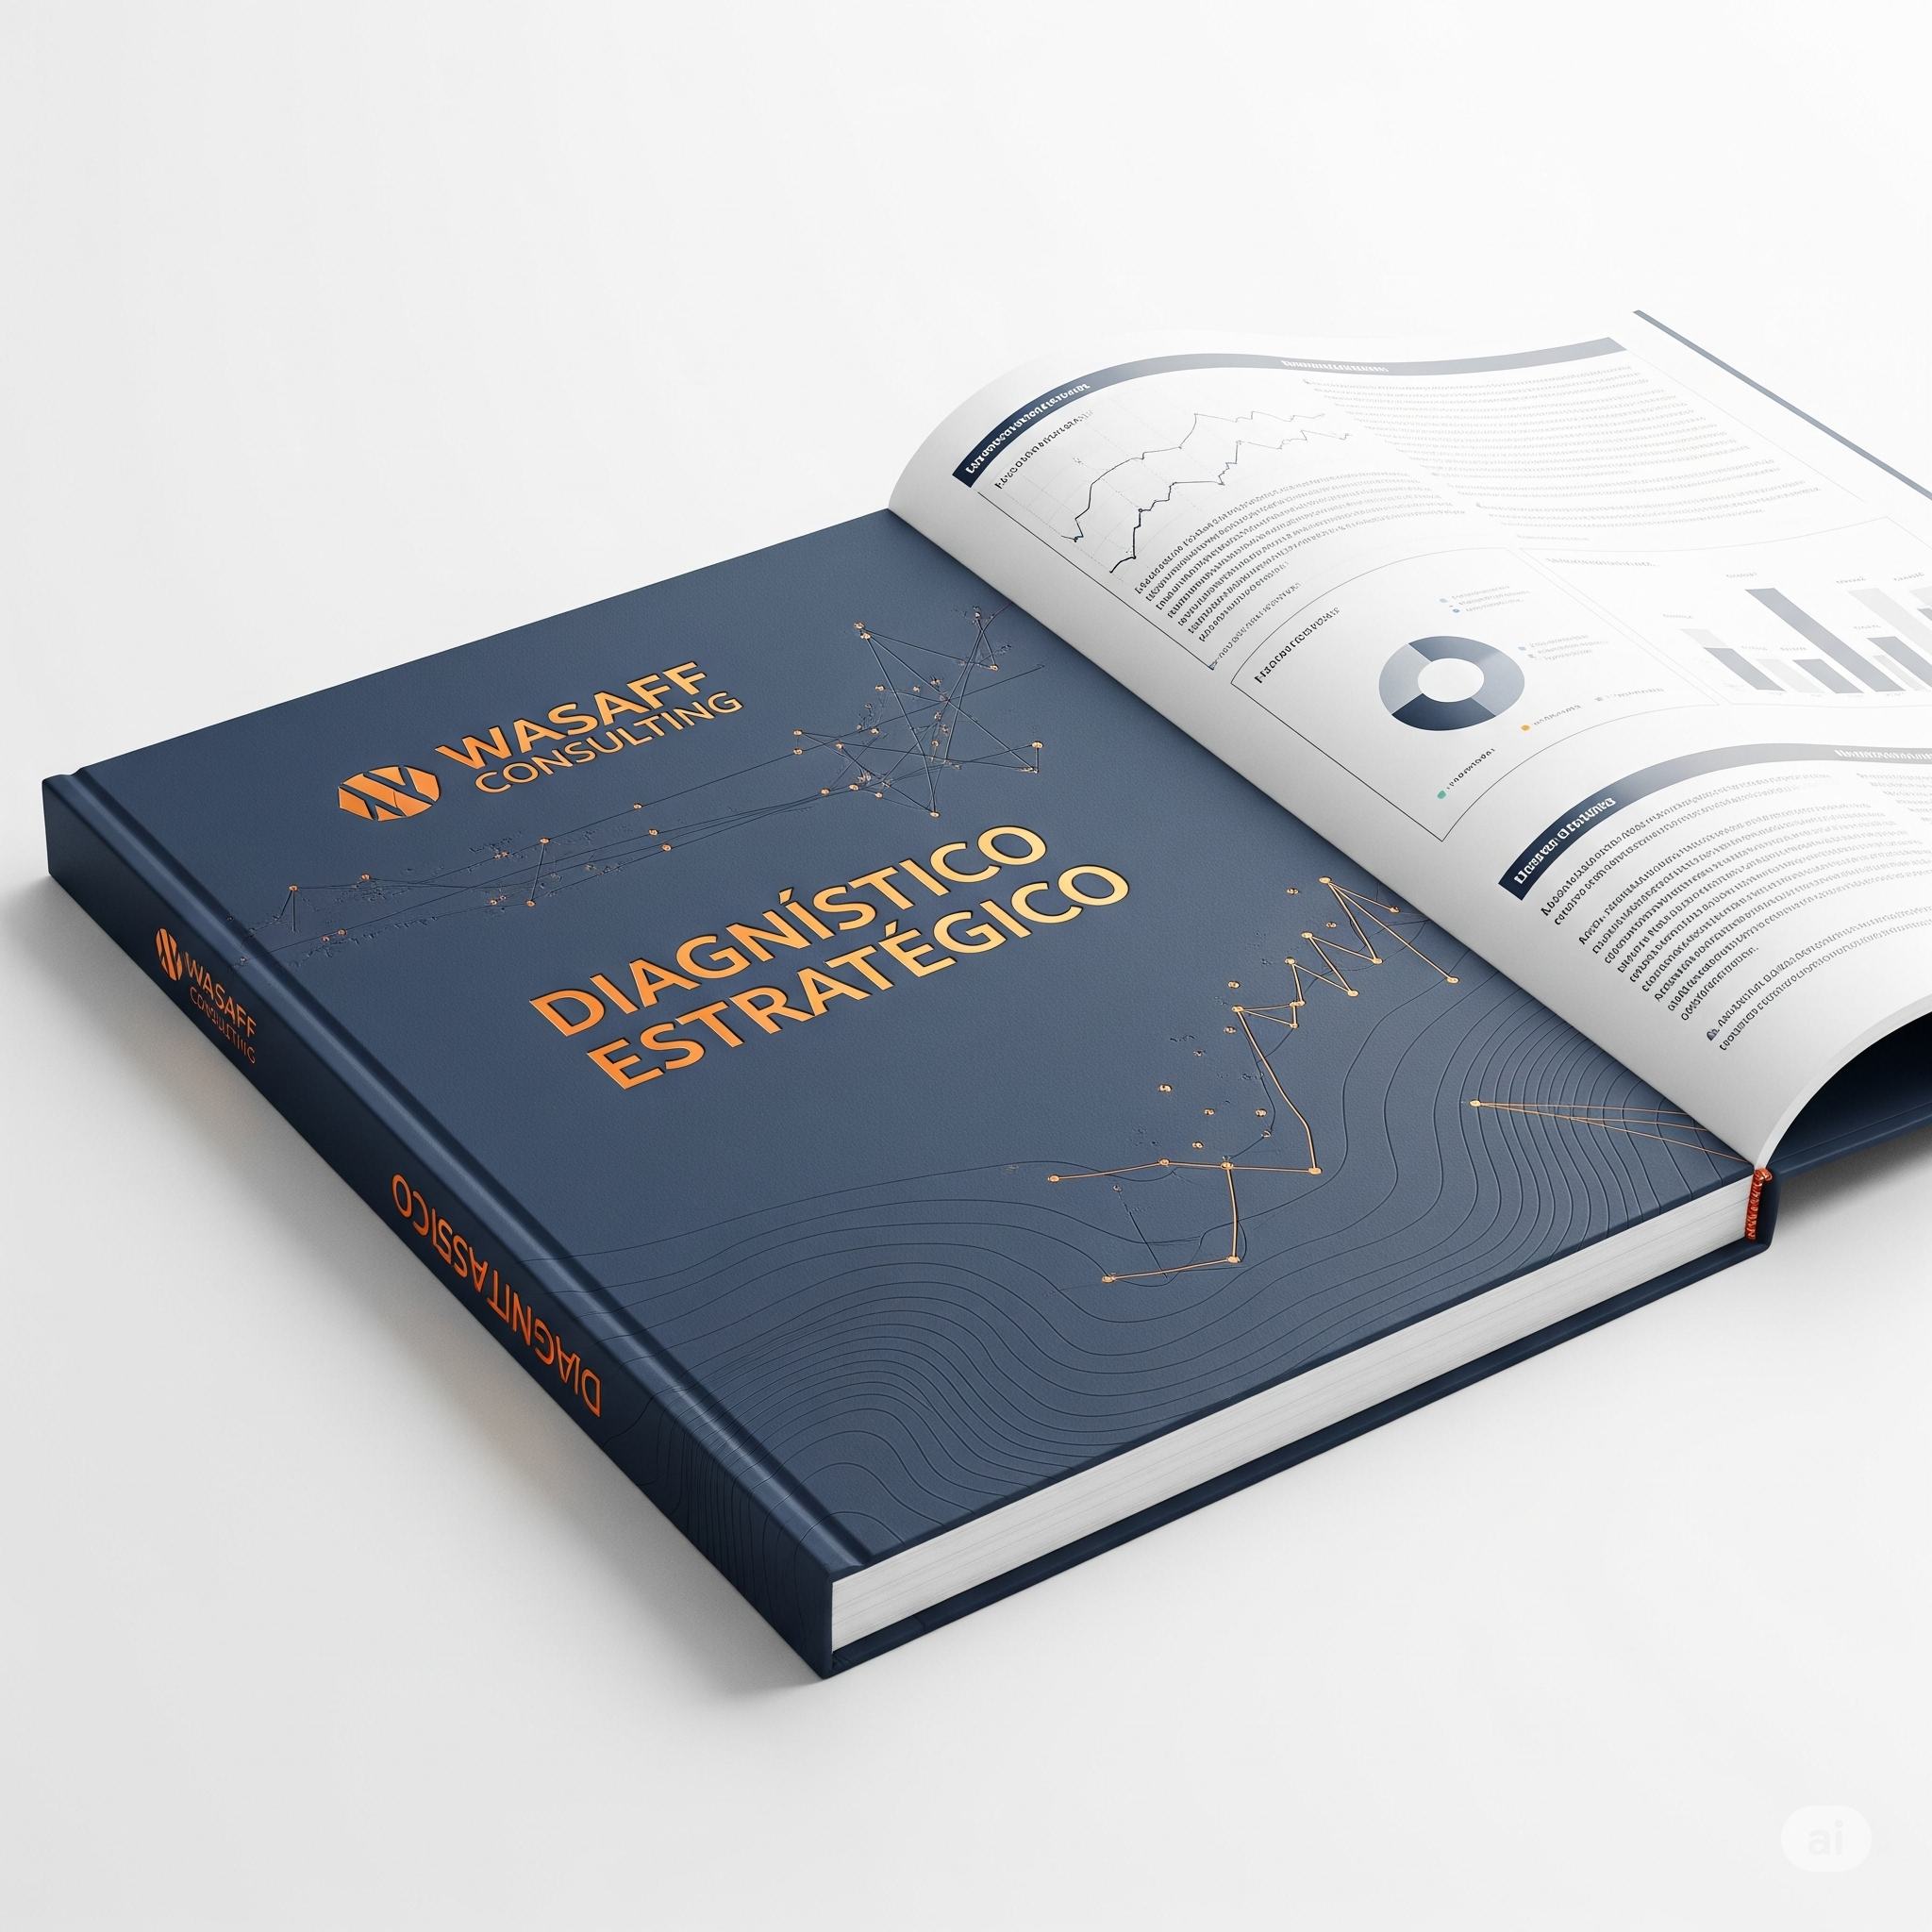
\includegraphics[scale=.05]{white_paper_cover.png} 
           \caption*{\small Informe Técnico Completo} 
      \end{figure}
      
      \begin{center}
          \qrcode[height=2.5cm]{https://www.wasaffconsulting.com/como-empezar}
          \\
          \tiny \textit{Agende su consulta}
      \end{center}
    \end{column}
  \end{columns}
\end{frame}

\end{document}